\chapter{Application requirements and specifications}
\label{chap:specs}

\par The main goal of the application is to create an alternative way of interacting with a live video. For this purpose a deep learning neural network is used trained on a custom hand gesture dataset. The machine learning algorithm will identify hand gestures, acting as the controlling tools for the application. 

\section{Application requirements}
\label{sec:specssec1}

\par The main focus of the application is the alternative way of interacting with the live video feed, providing features for drawing on the video and clearing it, for toggling mute and for incrementally changing the audio level up and down using simple hand gestures shown in chapter \ref{chap:model}.
\par Besides the drawing and clearing functionalities all others have a specific buttons and sliders as well, allowing the user to completely ignore the machine learning part if they choose to. In that case the application works as simple video recording tool with settings options for camera and microphone input and path choices for video and screenshot folders. This is shown in a more compact and visual way in the use case diagram below \ref{fig:usecase}, which was created with the help of an online diagram creation tool called Lucidchart \cite{lucidchart}.

\begin{figure}
    \centering
    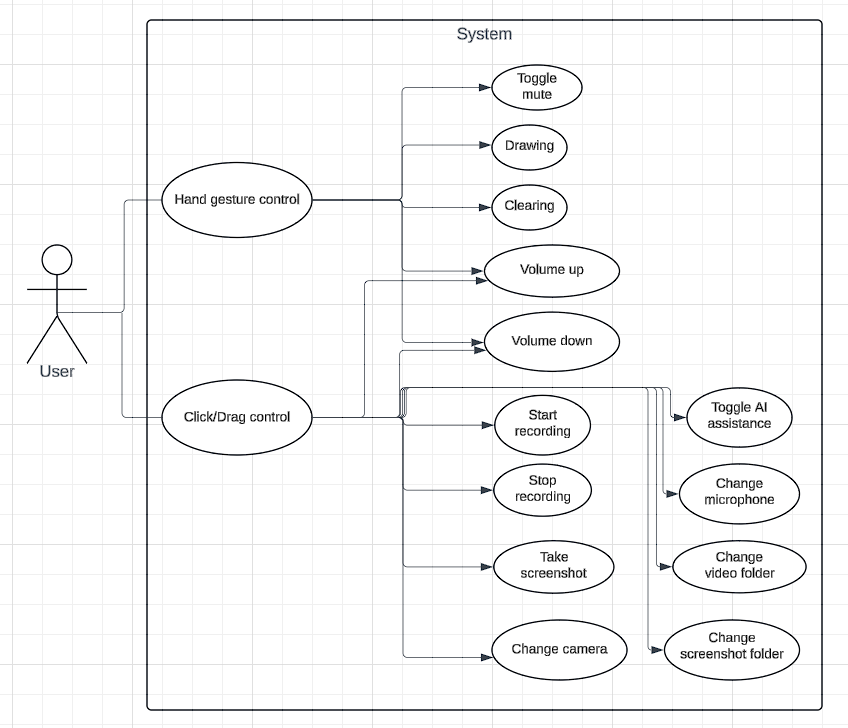
\includegraphics[width=0.6\linewidth]{figures/UseCaseDiagram.png}
    \caption{Use case diagram for the functionalities of the application}
    \label{fig:usecase}
\end{figure}

\subsection{Functional requirements}
\label{sec:specssec1subsec1}

\par To see the functionalities of the applications in an easier way, all of the above mentioned features are represented and described as use cases. The list with them is presented in Table\ref{UseCaseTable}, while the descriptions will be in the ones after.

\begin{table}[htbp]
\begin{center}
\begin{tabular}
{|p{90pt}|p{270pt}|}
\hline
 Use Case & Name\\
\hline 
\hline F1 & Start recording \\
\hline F2 & Stop recording \\
\hline F3 & Take screenshot \\
\hline F4 & Change volume up \\
\hline F5 & Change volume down \\
\hline F6 & Change video folder path \\
\hline F7 & Change screenshot folder path \\
\hline F8 & Change camera used during recording \\
\hline F9 & Change microphone used during recording \\
\hline F10 & Toggle artificial intelligence assistance \\
\hline F11 & Draw during recording \\
\hline F12 & Clear screen after drawing \\
\hline F13 & Toggle being muted \\
\hline
\end{tabular}
\end{center}
\caption{The application's functionalities represented as use cases}
\label{UseCaseTable}
\end{table}

\subsection{Functional requirements descriptions}
\label{sec:specssec1subsec1d1}

\par The F1 requirement is responsible for starting the video capture process. The steps and requirements for this functionality can be found in the table below \ref{F1Table}.
\par Prerequisites: The user chose a functioning camera and microphone; The user chose a path for the video to be saved in.
\par Post: The live feed of the video recording shows up on the screen; A pop-up message is shown to inform the user that the recording has started and in case the recording could not be started.

\begin{table}[htbp]
\begin{center}
\begin{tabular}
{|p{180pt}|p{180pt}|}
\hline
 User & System\\
\hline 
\hline 1. The user presses the Start button &  \\
\hline  & 2. The system checks for a functioning camera and microphone \\
\hline  & 3. The system checks if the folder path given exists or not \\
\hline  & 4 The system starts the video capture \\
\hline  & 4.1 The system presents the live feed on the screen with appropriate message\\
\hline  & 4.2 The system shows a pop-up error message about the failure at start or during recording \\
\hline
\end{tabular}
\end{center}
\caption{F1 Functionality steps}
\label{F1Table}
\end{table}

\par The F2 requirement is responsible for stopping the video capture process. The steps and requirements for this functionality can be found in the table below \ref{F2Table}.
\par Prerequisites: The video recording is running successfully.
\par Post: The live feed on the screen will stop and turn into a black image and the video is present in the chosen folder; A pop-up message is shown about the stop.

\begin{table}[htbp]
\begin{center}
\begin{tabular}
{|p{180pt}|p{180pt}|}
\hline
 User & System\\
\hline 
\hline 1. User presses the Stop button &  \\
\hline  & 2. The system stops the recording \\
\hline  & 3. The system creates the final video file in the selected folder \\
\hline  & 4 A black image is shown instead of the live feed and appropriate message is presented\\
\hline
\end{tabular}
\end{center}
\caption{F2 Functionality steps}
\label{F2Table}
\end{table}

\par The F3 requirement is responsible for taking a screenshot from the live feed. The steps and requirements for this functionality can be found in the table below \ref{F3Table}.
\par Prerequisites: The video recording is running successfully; A valid path is chosen as the screenshot folder.
\par Post: A pop-up message shows the screenshot was successfully taken and the picture will be present in the given folder; A pop-up message is shown in case of success and error.

\begin{table}[htbp]
\begin{center}
\begin{tabular}
{|p{180pt}|p{180pt}|}
\hline
 User & System\\
\hline 
\hline 1. User presses the Screenshot button &  \\
\hline  & 2. The system saves the last frame in the chosen folder \\
\hline  & 3.1 A pop-up message is shown when successful \\
\hline  & 3.2 The system shows a pop-up error message about the failure \\
\hline
\end{tabular}
\end{center}
\caption{F3 Functionality steps}
\label{F3Table}
\end{table}

\par The F4/F5 requirements are responsible for changing the volume down and up respectively. The steps and requirements for these functionalities can be found in the table below \ref{F5Table}.
\par Prerequisites: The volume is not at 0 percent(down)/100 percent(up); For hand gesture control the recording is running and the AI assistance is turned on.
\par Post: The volume of the audio will be changed in the current or next recording.

\begin{table}[htbp]
\begin{center}
\begin{tabular}
{|p{180pt}|p{180pt}|}
\hline
 User & System\\
\hline 
\hline 1.1 The user moves the volume slider to the left(down)/right(up) &  \\
\hline 1.2 The user show the second(down)/first(up) hand gesture in figure \ref{customDataset} &  \\
\hline  & 2. The system saves the volume modifier accordingly \\
\hline
\end{tabular}
\end{center}
\caption{F4/F5 Functionality steps}
\label{F5Table}
\end{table}

\par The F6/F7 requirements are responsible for changing the folder path for the video/screenshot files. The steps and requirements for these functionalities can be found in the table below \ref{F7Table}.
\par Prerequisites: The video recording is not running.
\par Post: The folder path for the video/screenshot files will be changed accordingly and the user is sent back to the main window.

\begin{table}[htbp]
\begin{center}
\begin{tabular}
{|p{180pt}|p{180pt}|}
\hline
 User & System\\
\hline 
\hline 1. The user presses the Settings button &  \\
\hline  & 2. The current window is changed to the Settings window \\
\hline 3. The user presses the "Choose Path" button in the Screenshot/Video folder path section&  \\
\hline  & 4. The windows File explorer opens \\
\hline 5. The user chooses a folder &  \\
\hline  & 6. The system changes the path to the chosen one without saving it \\
\hline 7. The user presses the Save button &  \\
\hline  & 8. The system saves the setting changes to the configuration file \\
\hline  & 9. The system switches back to the main window \\
\hline
\end{tabular}
\end{center}
\caption{F6/F7 Functionality steps}
\label{F7Table}
\end{table}

\par The F8/F9 requirements are responsible for changing the used camera/microphone. The steps and requirements for these functionalities can be found in the table below \ref{F9Table}.
\par Prerequisites: The video recording is not running.
\par Post: The chosen camera/microphone to be in use will be changed and the user is sent back to the main window.

\begin{table}[htbp]
\begin{center}
\begin{tabular}
{|p{180pt}|p{180pt}|}
\hline
 User & System\\
\hline 
\hline 1. The user presses the Settings button &  \\
\hline  & 2. The current window is changed to the Settings window \\
\hline 3. The user presses the drop-down list in the Camera/Microphone section&  \\
\hline  & 4. The systems shows a list of available cameras/microphones \\
\hline 5. The user chooses a camera/microphone from the list &  \\
\hline  & 6. The system changes the camera/microphone to the chosen one without saving it \\
\hline 7. The user presses the Save button &  \\
\hline  & 8. The system saves the setting changes to the configuration file \\
\hline  & 9. The system switches back to the main window \\
\hline
\end{tabular}
\end{center}
\caption{F8/F9 Functionality steps}
\label{F9Table}
\end{table}

\par The F10 requirement is responsible for toggling the AI assistance during video recording. The steps and requirements for this functionality can be found in the table below \ref{F10Table}.
\par Prerequisites: None.
\par Post: The AI assistance will be toggled on or off.

\begin{table}[htbp]
\begin{center}
\begin{tabular}
{|p{180pt}|p{180pt}|}
\hline
 User & System\\
\hline 
\hline 1. The user checks or unchecks the AIAssistance button &  \\
\hline  & 2. The system toggles the feature on or off \\
\hline
\end{tabular}
\end{center}
\caption{F10 Functionality steps}
\label{F10Table}
\end{table}

\par The F11 requirement is responsible for hand gesture driven drawing during video recording. The steps and requirements for this functionality can be found in the table below \ref{F11Table}.
\par Prerequisites: The video recording is running and the AI assistance is turned on.
\par Post: Given a specific hand gesture the system draws on the video feed following the users finger, visible both on the live feed and in the recording.

\begin{table}[htbp]
\begin{center}
\begin{tabular}
{|p{180pt}|p{180pt}|}
\hline
 User & System\\
\hline 
\hline 1. The user shows the fourth hand gesture in figure \ref{customDataset} &  \\
\hline  & 2. The system whitens the pixels in a small radius near the end of the fingers of the user \\
\hline
\end{tabular}
\end{center}
\caption{F11 Functionality steps}
\label{F11Table}
\end{table}

\par The F12 requirement is responsible for clearing the video feed of any drawing during recording. The steps and requirements for this functionality can be found in the table below \ref{F12Table}.
\par Prerequisites: The video recording is running and the AI assistance is turned on.
\par Post: Given a specific hand gesture the system clears the video feed of any drawing.

\begin{table}[htbp]
\begin{center}
\begin{tabular}
{|p{180pt}|p{180pt}|}
\hline
 User & System\\
\hline 
\hline 1. The user shows the fifth hand gesture in figure \ref{customDataset} &  \\
\hline  & 2. The system clears the video feed of any hand drawing \\
\hline
\end{tabular}
\end{center}
\caption{F12 Functionality steps}
\label{F12Table}
\end{table}

\par The F13 requirement is responsible for toggling being muted via hand gesture during video recording. The steps and requirements for this functionality can be found in the table below \ref{F13Table}.
\par Prerequisites: The video recording is running and the AI assistance is turned on.
\par Post: Given a specific hand gesture the system toggles between being muted and the previous audio level.

\begin{table}[htbp]
\begin{center}
\begin{tabular}
{|p{180pt}|p{180pt}|}
\hline
 User & System\\
\hline 
\hline 1. The user shows the third hand gesture in figure \ref{customDataset} &  \\
\hline  & 2. The system toggles between being muted and the previous audio level before the mute \\
\hline
\end{tabular}
\end{center}
\caption{F13 Functionality steps}
\label{F13Table}
\end{table}

\subsection{Non-functional requirements}
\label{sec:specssec1subsec2}

\par The processing of the input images from the video feed is done in real-time with the frame rate being determined by the input camera. The hand gesture identification and finger tracking is done on every couple frame, depending on the frame rate of the recording in the current moment.
\par The saving of the video files and images are done by only accessing those particular folders, with a naming convention of Recording\\Screenshot with the current date and time, so conflicts with other existing files is almost impossible, at the very least highly unlikely.

\subsection{System requirements}
\label{sec:specssec1subsec3}

\par The application needs a working camera and microphone and it only runs on the Windows operating system, 10 or 11 64-bit version, running on other versions may result in undefined behaviour.
\par By testing the application on a Ryzen 7 4800h and NVIDIA GeForce GTX 1660 Ti, 8 and 30 percent being used respectively, the minimum requirements are Intel Core i7-9750h and a dedicated NVIDIA video card for a smooth experience. The application can run solely on CPU as well, but in that case the lag might too much for a watchable video. In terms of RAM the application needs a minimum of 2600 MB, more is necessary depending on the length of the recording.
\par In order to run the application using the graphics card the 11.2 version of CUDA has to be installed and setup up, which is a tool developed by NVIDIA for general parallel programming on their GPUs.
\par In terms of storage, the application only needs around 300 Megabytes. The real impact will come from the saved video and screenshot files.

\label{sec:specssec2}

\section{Technical specifications}
\label{sec:specssec2}

\par For the purpose of easier integration of the deep learning model, the language used to develop the application is python, where most frameworks used for machine learning are written.
\par For creating and working with the SSD MobileNet architecture, I use the TensorFlow \cite{tensorflow2015-whitepaper} framework. TensorFlow is an open-source project developed by Google giving an easy API for developing machine learning models efficiently, by wrapping up the more complex C++ and CUDA core functionalities.
\par The opencv library \cite{opencv_library} is used for capturing and working with visuals. It is open-source computer vision library written in mostly C++ and it is often used in computer vision projects, making the integration with the model easier. The pyaudio module \cite{pyaudio}, a cross-platform library, is used for capturing the audio, while the wave module \cite{wave} is used for saving it.  
\par For the creation of the graphical user interface, the cross-platform Qt framework is used \cite{QtPage}. With the help of this library interfaces can be built in a modular fashion, making development easier and it is written in C++, which provides good performance.
\par Besides the major libraries, the win32api package \cite{win32api} is also used to access certain computer specifications, like the width and height of the monitor screen, for aligning the application at launch. To store the settings of the user, the json format is used, with the help of the json library \cite{jsonlib}, so the structure of the storage is easy to read for both the application and the user, in case a manual change would be needed.